
\begin{tikzpicture}

% for double arrows a la chef
% adapt line thickness and line width, if needed
\tikzstyle{vecArrow} = [thick, fill=white, decoration={markings,mark=at position
	1 with {\arrow[semithick]{open triangle 60}}},
double distance=1.4pt, shorten >= 5.5pt,
preaction = {decorate},
postaction = {draw,line width=1.4pt, white,shorten >= 4.5pt}]
\tikzstyle{innerWhite} = [semithick, draw=white,line width=1.4pt, shorten >= .5pt]

\node[inner sep=0pt] (x1) at (0,0)
    {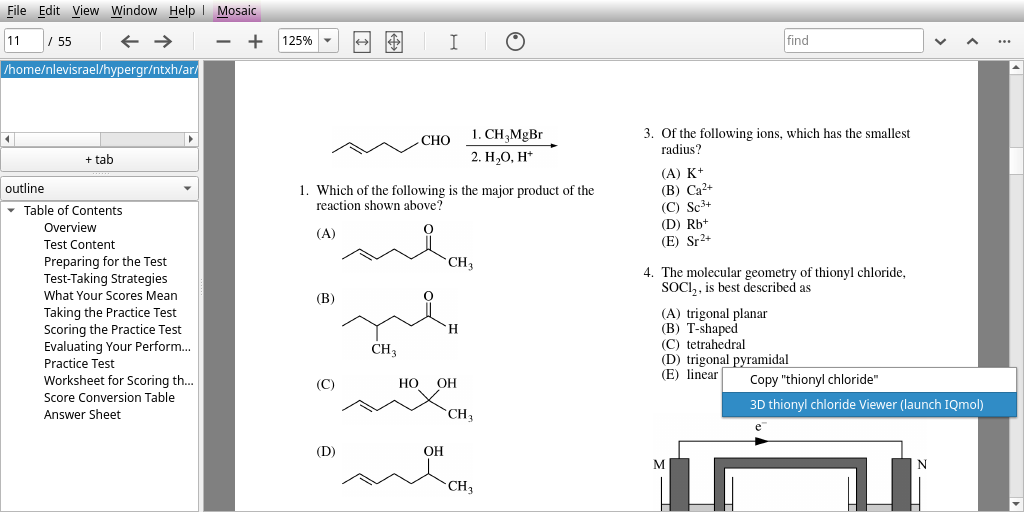
\includegraphics[width=110mm, 
    	trim={30mm 0 0 30mm},clip]
    	{xScreenShot2.png}};
    
%\node[inner sep=0pt] (icon) at (4.5,-1.44)
%    {
\includegraphics[width=2.7mm]{cursor-4.png}};
    
\node (apos) at (4.8,-1.7){};
\node (pos) at (4.4,-1.04){};

\node at (4.4,-1.44) [
    draw=black,
    %minimum width=2ex,
    inner sep=.7pt,
    fill=white,
    single arrow,
        single arrow head extend=3pt,
        single arrow head indent=1.5pt,
        single arrow tip angle=45,
        line join=bevel,
    minimum height=4.6mm,
    rotate=115
] {};

%\draw[vecArrow] (apos) to (pos);
%\draw[innerWhite] (apos) to (pos);

    
%    {
\includegraphics[width=2.7mm]{computer-arrow-png-2.png}};
%    {
\includegraphics[width=3.7mm]{curser-png-7.png}};
%    {
\includegraphics[width=4.3mm]{cursor-icon-png-14}};
%    {
\includegraphics[width=2.7mm]{cursor-arrow.png}};
%    {
\includegraphics[width=3.2mm]{mv2.png}};


\end{tikzpicture}

